\documentclass[conference]{IEEEtran}
\IEEEoverridecommandlockouts
% The preceding line is only needed to identify funding in the first footnote. If that is unneeded, please comment it out.
\usepackage{cite}
\usepackage{amsmath,amssymb,amsfonts}
\usepackage{algorithmic}
\usepackage[pdftex]{graphicx}
\usepackage{textcomp}
\usepackage{xcolor}
\usepackage{kotex}
\usepackage{href-ul}
\usepackage{float}
\def\BibTeX{{\rm B\kern-.05em{\sc i\kern-.025em b}\kern-.08em
    T\kern-.1667em\lower.7ex\hbox{E}\kern-.125emX}}
\begin{document}

\newcommand{\libpng}{\textbf{libpng}}
\newcommand{\Eigen}{\textbf{Eigen}}
\newcommand{\Qt}{\textbf{Qt}}

\newcommand{\eg}{\textbf{eg}}
\newcommand{\egExceptions}{\textbf{egExceptions}}
\newcommand{\egGeometry}{\textbf{egGeometry}}
\newcommand{\egLoader}{\textbf{egLoader}}
\newcommand{\egMath}{\textbf{egMath}}
\newcommand{\egMethods}{\textbf{egMethods}}
\newcommand{\egOperators}{\textbf{egOperators}}
\newcommand{\egProcessing}{\textbf{egProcessing}}
\newcommand{\egTrace}{\textbf{egTrace}}
\newcommand{\egTypes}{\textbf{egTypes}}
\newcommand{\egTool}{\textbf{egTool}}

\newcommand{\imgascii}{\textbf{img2ascii}}
\newcommand{\tone}{\textbf{tone}}
\newcommand{\structure}{\textbf{structure}}

\title{AAC(Ascii Art Converter)\\ \vspace{1em}
{\large 2023 2학기, CSE2035/AIE2051 \\ 서강대학교 \\} \vspace{0.5em}
{
\includegraphics[width=1.5cm]{./sogang_university_logo.png}}
{\large ~\\~}
{\large \\ 기말 프로젝트 \\ Team: No More Double \\ \vspace{-1em}\href{https://github.com/arduinocc04/AAC}{https://github.com/arduinocc04/AAC}}}
\author{\IEEEauthorblockN{1\textsuperscript{st} 조다니엘}
\IEEEauthorblockA{\textit{컴퓨터공학과} \\
danielcho@sogang.ac.kr}
\and
\IEEEauthorblockN{2\textsuperscript{nd} 박준영}
\IEEEauthorblockA{\textit{컴퓨터공학과} \\
sparkjy18@sogang.ac.kr}}

\begin{figure}
    \hspace{2.25em}
    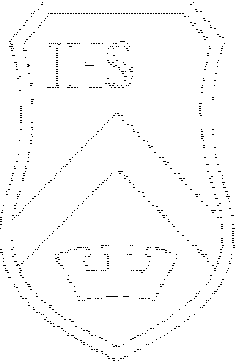
\includegraphics[width=0.75\paperwidth]{ascii_logo_1.pdf}
\end{figure}

\maketitle

\begin{abstract}
AAC(Ascii Art Converter)는 png 이미지 파일을 아스키 아트로 변환하여 출력하는 프로그램이다.
이미지 변환 방식은 크게 tone-based 방식과 structure-based 방식으로 나뉜다.
tone-based 방식은 이미지의 각 픽셀의 rgba 값을 읽어들인 후 red, green, blue 값의 평균으로 픽셀의 밝기를 결정하여 색조 이미지를 회색조로 변환한다.
이후 픽셀의 밝기 정도에 따라 그에 해당하는 아스키 문자로 픽셀을 변환하여 출력한다.
structure-based 방식은 이미지를 회색조로 변환한 뒤 convolution 연산을 활용한 edge-detection 알고리즘을 적용하며, morphology 또는 Gaussian-blur 연산을 적용하여 정제된 결과를 얻는다.
이후 Suzuki 알고리즘을 사용하여 외곽선을 추출한 후 외곽선의 곡선을 선분으로 분할하여 이미지를 벡터화한다.
최종적으로 벡터화된 이미지를 그리드로 분할한 다음 그리드별로 log-polar 히스토그램을 얻고, Bhattacharyya 거리를 이용하여 가장 유사한 아스키 문자를 선택한다.
이 과정에서 simulated annealing 기법을 이용해 이미지가 아스키 아트로 잘 표현되도록 이미지를 변형하였다.
\end{abstract}

\section{동기}
\begin{description}
    \item[박준영]: YouTube에서 접했던 donut.c\cite{b1} 아스키 아트를 보고 비슷하게 이미지 변환을 구현해 보고자 시작하였다.
    \item[조다니엘]\hspace{1em}: AAC(악)이라는 프로그램의 이름이 마음에 들었다.
\end{description}

\section{프로젝트 구조}

\subsection{\eg}

\eg는 \textbf{E}asy pn\textbf{G}의 줄임말로 오픈 소스 라이브러리 \libpng와 \Eigen을 사용하여 구현한 라이브러리이다.
\eg는 이미지 변환에 필요한 연산을 담당하는 \egGeometry, \egMath, \egMethods, \egOperators, \egProcessing, \egTrace, \egTool과 그 밖의 이미지 입출력, 타입 정의, 에러 핸들링을 담당하는 \egLoader, \egTypes, \egExceptions로 구분된다.

\subsubsection{\egLoader}

\egLoader 에는 png 파일을 읽고, 저장하는데 도움을 주는 \libpng를 이용하여 png 이미지 파일의 가로, 세로 및 rgba 값을 읽어들인 다음 각각 텐서의 원소로 저장한다.
또한 \Eigen 텐서 형태로 저장되어 있는 Image를 다시 png 파일로 export하는 기능이 내장되어 있다.

\subsubsection{\egMethods}

\egMethods는 지원 가능한 이미지 연산, 변환 방법을 enum 타입으로 정의한 파일이다.
대표적으로 색조 변환, blur, 외곽선 추출 등이 있다.

\subsubsection{\egMath}

\egMath는 edge-detection에 활용되는 convolution 연산, 행렬 간의 거리를 비교하는 RMSE, shape-context, log-polar 좌표계 변환 연산, 히스토그램 간의 거리를 비교하는 Bhattacharyya 연산이 포함되어 있다.

\subsubsection{\egGeometry}

\egGeometry는 시계/반시계 방향을 판단하는 ccw() 함수 및 점과 선분 사이의 거리를 계산하는 distSegDot() 함수, 내적 및 외적, 유클리드 좌표계의 거리와 log-polar 좌표계의 거리를 계산하는 함수들이 내장되어 있다. 

\subsubsection{\egProcessing}

\egProcessing은 이미지 처리와 관련된 전반적인 구현이 모두 포함되어 있다.
색조 이미지를 회색조로 변환하는 cvtGray(),
외곽선을 추출하는 getEdge(),
blur 처리를 담당하는 blur(),
grassfire 알고리즘을 활용하여 중심선을 추출하는 extractCenterline(),
0과 255 사이를 벗어나는 밝기 값을 범위 안으로 축소하는 saturate(),
일정 역치를 벗어나는 이미지의 명도 픽셀 값을 표시하는 markOutlier(),
binary 이미지의 0과 1값을 반전시키는 reverse(),
이미지 morphology 연산에 활용하기 위하여 구현한 erode() 및 dilate(),
Suzuki 알고리즘을 이용하여 외곽선을 추출하는 getContours(),
log-polar 좌표계를 이용하여 히스토그램을 얻는 logpolar(),
외곽선을 선분으로 분할하는 drawSegments() 함수 등이 있다.

\subsubsection{\egTrace}

\egTrace는 approxPath() 등 점을 선분으로 근사하는 함수를 사용하여 이미지의 외곽선을 여러 개의 선분으로 재분류한다.

\subsubsection{\egTool}

\egTool은 line clipping 과정에서 사용되는 Cohen–Sutherland 알고리즘\cite{cohen-sutherland}과 점을 선분으로 합치는 merge() 함수가 구현되어 있다.

\subsubsection{\egTypes}

\egTypes에는 프로젝트에서 사용하기 위해 새롭게 정의한 타입들의 정보를 한데 모아 놓았다.

\subsubsection{\egOperators}

\egOperators에는 픽셀의 x좌표, y좌표를 각각 더하고 빼거나 부호를 반전할 수 있도록 연산자 오버로딩을 정의해 놓았다.

\subsubsection{\egExceptions}

\egExceptions는 프로그램을 실행 중에 오류가 발생하면 에러 코드를 throw하고 작동을 멈춤으로써 프로그램의 undefined behavior를 방지하는 역할을 한다.

\subsection{\imgascii}

\imgascii는 \eg 라이브러리를 바탕으로 이미지를 아스키 아트로 변환하는 과정을 기술한 소스코드이다.
tone-based 방식으로 변환하는 \tone과 structure-based 방식으로 변환하는 \structure로 나뉜다.

\subsubsection{\tone}
tone-based 방식 변환은 회색조 변환 단계 이후 각 픽셀별 red, blue, green 값의 평균을 이용하여 밝기를 추출하고, 해당 밝기의 정도에 따라 문자를 선택하여 출력한다.

\subsubsection{\structure}

\section{프로그램의 동작}

이번 절에서는 structure-based 방식의 이미지 변환을 설명한다.

\subsection{이미지 파일의 입력}

이미지 파일을 입력받는다. 이미지 파일의 형식이 png인지 확인하고, 형식에 맞지 않는 이미지 파일을 받으면 오류를 발생시킨다.
\egLoader에 구현된 PNG 클래스를 활용하였으며, 특히 openImage() 메서드를 중점적으로 사용하였다.

\subsection{이미지 전처리}

\subsubsection{회색조 변환}

색조 이미지의 red, green, blue 값의 평균을 구하여 픽셀의 밝기를 도출한 뒤 회색조 이미지로 변환한다.

\subsubsection{1차 외곽선 추출}

회색조로 변환된 이미지의 외곽선을 추출한다.

\subsubsection{Blurring or Morphology}

Gaussian-blur 또는 dilate, erode 연산을 이용하여 이미지의 노이즈를 줄인다.

\subsubsection{Binary 변환}

이미지를 공백에 해당하는 0과 선에 해당하는 1로 표현하여 2차원 행렬에 저장한다.
일정 역치를 설정하여 역치를 넘기지 못하는 밝기의 픽셀은 0, 넘기는 밝기의 픽셀은 1로 저장한다.

\subsubsection{2차 외곽선 추출}
Suzuki의 알고리즘\cite{suzuki}을 이용하여 외곽선을 추출한다.

\subsubsection{외곽선의 선분 분할}
suzuki의 알고리즘을 이용하면 이차원 행렬의 각 점이 어떤 외곽선에 속해있는지 알아낼 수 있다.
이를 바탕으로 같은 외곽선에 있는 점을 시계방향 또는 반시계방향으로 정렬하여 외곽선을 선분으로 분할하여 이미지를 벡터화한다.
위의 사항을 구현하기 위하여 자체 제작한 알고리즘이 사용되었다. 
\begin{enumerate}
    \item 왼쪽 위 $(0, 0)$부터 오른쪽 아래 $(H, W)$ 방향으로 행렬의 각 원소를 검사한다. \label{B61}
    \item 만약 해당 픽셀을 포함하는 외곽선이 이전에 검사된 적이 있거나 픽셀의 값이 0 이라면 \ref{B61}로 돌아간다.
    \item 현재 픽셀의 왼쪽 아래에 위치한 픽셀부터 시계 반대 방향으로 자신과 같은 외곽선에 속한 픽셀을 찾는다. 없다면 \ref{B61}로 돌아간다. \label{B63}
    \item 연결된 픽셀을 순차적으로 탐색하며 연결된 픽셀이 더 이상 없을 때까지 스택에 픽셀의 좌표를 넣는다.
    \item 스택을 뒤집는다.
    \item \ref{B63}에서 얻은 픽셀의 시계 반대 방향에 위치한 다음 픽셀부터 시계 반대 방향으로 탐색을 시작한다.
    만약 기존에 방문한 픽셀밖에 없거나, 같은 외곽선에 속한 픽셀을 찾을 수 없다면 \ref{B61}로 되돌아간다.
    \item 다시 아직 방문하지 않은 연결된 픽셀을 순차적으로 탐색하여, 연결된 픽셀이 더 이상 없을 때까지 스택에 픽셀의 좌표를 넣는다. 이후 \ref{B61}로 돌아간다.
\end{enumerate}
\begin{figure}
    \centering
    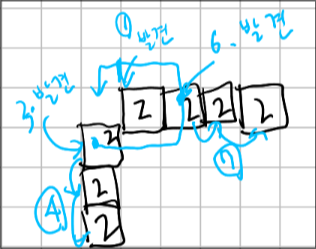
\includegraphics[width=6cm]{algo.png}
    \caption{점의 집합을 시계 방향 또는 시계 반대 방향으로 정렬하는 알고리즘}
\end{figure}
위의 과정이 끝나면 그리디 알고리즘을 이용하여 점들을 선분으로 근사한다.
선분$\overline{A_1A_2}$와 점 $P$ 사이의 거리는 식 \ref{eq:distDotSeg}\로 정의한다.
\begin{equation}
    \begin{cases}
        \overline{A_1P} & \text{If } (A_2 - A_1) \cdot (P - A_1) \leq 0 \\
        \overline{A_2P} & \text{If } (A_1 - A_2) \cdot (P - A_2) \leq 0 \\
        \frac{|(P - A_1)\times (A_2 - A_1)|}{\overline{A_1A_2}} & \text{otherwise}
    \end{cases}
    \label{eq:distDotSeg}
\end{equation}
시계 방향 또는 시계 반대 방향으로 정렬된 점들의 배열 $A$가 주어졌을 때, 어떤 $i < j$인 음이 아닌 정수 $i, j$에 대하여,
선분 $\overline{A_iA_j}$와 점 $A_k$($i < k < j$)의 거리가 $\sqrt 2 \approx 1.42$ 이하라면, $i$에서 $j$번째까지의 점들이 선분으로 근사되었다고 판단하였다.
위의 기준을 이용하여 배열의 앞쪽부터 점들을 순회하면서 기존의 선분에 포함할 수 있다면 포함하고, 그렇지 않다면 새로운 선분을 생성하였다.

\subsection{이미지 최적화}

\subsubsection{선분을 그리드로 분할}
Cohen-Sutherland 알고리즘\cite{cohen-sutherland}을 사용하여 길이가 긴 선분을 일정한 간격의 그리드로 분할하였다.

\subsubsection{Simulated Annealing}
임의의 정점을 조금씩 움직이면서 Bresenham's line algorithm\cite{bresenham-line}을 사용해 그림을 새로 그렸다.
이후 이미지가 아스키 아트를 더 잘 표현하는 결과물로 변화하였는지 확인한다.
주어진 그리드에 어떤 문자가 가장 잘 대응되는지 판단하기 위하여 좌표계를 log-polar coordinate로 변환한 후 히스토그램을 만들어 Bhattacharyya 거리를 비교하여 판단하였다.\cite{st-ba-ascii-art}


\section{프로젝트 진행 과정}

프로젝트의 첫 계획은 이미지를 아스키 아트로 변환하는 프로그램과 변환된 아스키 아트를 출력하는 프로그램 두 가지를 결합하는 형식이었다.
그러나 \Qt로 뷰어를 구현하는 과정이 지루하였기 때문에 아스키 아트 변환에만 집중해서 프로젝트를 진행하기로 결정하였다.
방식을 일반적으로 널리 알려지고 구현 난도도 낮은 tone-based 방식과 구현 난이도가 높지만 훨씬 만족스러운 결과를 도출하는 structure-based 방식으로 나누어 각자 구현하기로 하였다. \\
\indent 우선 \libpng가 제공하는 일련의 이미지 입출력 과정이 번거로워 이미지를 쉽고 빠르게 입출력할 수 있도록 \libpng의 메서드를 한데 모아 사용자 라이브러리를 만들었다.
그 다음 본격적으로 이미지 변환에 필요한 연산을 구현하려 하였는데, 처음에는 \libpng를 제외하고 아무런 오픈 소스 라이브러리를 사용하지 않으려 했다.
그러나 \libpng만으로는 이미지 상태 관리와 연산에 한계를 느껴 \Eigen을 도입하였다.
그 결과 이미지를 행렬과 텐서의 형태로 관리하여 한 픽셀을 텐서의 원소 하나에 일대일 대응시킴으로써 자연스럽게 convolution 등의 연산을 구현할 수 있었다.
또한 단순히 이중 반복문을 사용할 때보다 \Eigen에서 지원하는 메서드과 클래스를 사용하였을 때 연산 속도가 훨씬 빨랐다.
이로부터 외부 라이브러리의 적절한 선택과 사용이 프로그램의 성능을 확연히 개선할 수 있다는 사실을 알 수 있다. \\
\indent 당초의 예상대로 tone-based 방식의 아스키 아트는 구현이 용이하였으나 structure-based 방식은 생각보다 매우 많은 연구가 이루어져 있어 다양한 방법으로 구현을 시도할 수 있었다.
따라서 각종 문헌과 논문을 참고하여 최대한 이상적인 결과물을 얻기 위해 여러 알고리즘과 이미지 변환 기법을 사용하였다.
위와 같은 시도를 통해 여러 방법론을 결합하여 질 좋은 아스키 아트를 제작하는 프로그램을 완성하였지만, 주어진 시간의 부족으로 인해 소스코드와 라이브러리가 잘 정돈되지 못한 점이 아쉽다.

\section{프로그램 사용법}
\begin{enumerate}
\item \begin{verbatim}sudo pacman -S libpng eigen\end{verbatim}
\item \begin{verbatim}git clone https://github.com/arduinocc04/AAC\end{verbatim}
\item \begin{verbatim}cd AAC\end{verbatim}
\item \begin{verbatim}./install.sh\end{verbatim}
\item \begin{verbatim}cd build \end{verbatim}
\item \begin{verbatim}img2ascii/structure/sa-structure non-hangul-images IMAGE_FILE\end{verbatim}
\end{enumerate}

\begin{thebibliography}{00}
\bibitem{b1} % donut.c
\bibitem{suzuki} % https://www.sciencedirect.com/science/article/abs/pii/0734189X85900167
\bibitem{monotone-chain} % https://en.wikibooks.org/wiki/Algorithm_Implementation/Geometry/Convex_hull/Monotone_chain
\bibitem{grassfire} % https://en.wikipedia.org/wiki/Grassfire_transform
\bibitem{cohen-sutherland} % https://en.wikipedia.org/wiki/Cohen%E2%80%93Sutherland_algorithm
\bibitem{st-ba-ascii-art} % https://dl.acm.org/doi/10.1145/1778765.1778789
\bibitem{bresenham-line} % https://en.wikipedia.org/wiki/Bresenham%27s_line_algorithm
\end{thebibliography}

\end{document}
